\documentclass[twocolumn]{article}

\usepackage{amssymb}
\usepackage{amsmath}
\usepackage{graphicx}
\usepackage{caption}
\usepackage{amsmath}
\usepackage{cleveref}
\usepackage{framed}

\crefname{box}{box}{boxes}
\newcounter{BoxCounter}
\crefalias{BoxCounter}{box}

\newenvironment{infobox}[1]%
  {\refstepcounter{BoxCounter}\framed {\bfseries Box~\arabic{BoxCounter}:~#1}\newline}%
  {\endframed}
\newcommand{\kOx}{\ensuremath{k_{\mathrm{ox}}}}
\newcommand{\kRed}{\ensuremath{k_\mathrm{red}}}

\DeclareMathOperator{\CV}{CV}

\graphicspath{{./files/}}

\title{Modeling dispersion in surface confined electrochemical reactions}
\author{Gavin Stewart}

\begin{document}
	
	\maketitle
	
	\section{Introduction}
	
	\section{Surface Confined model}
	We consider the surface confined reaction described in \cref{eqn:surf-reaction} where the species $A$ is reduced to yield a new species $B$.
	\begin{equation}\label{eqn:surf-reaction}
		A + e^- \mathop{\rightleftarrows}^{\kOx}_{\kRed} B
	\end{equation}
	where the rates $\kOx$ and $\kRed$ are governed by the Butler-Volmer dynamic laws given in \cref{eqn:butler-volmer-rates}:
	\begin{equation} \label{eqn:butler-volmer-rates}
		\begin{aligned}
			\kRed(t) &= k_0 \exp\left(-\frac{\alpha F}{RT}[E_r(t) - E_0]\right)\\
			\kOx(t) &= k_0 \exp\left((1-\alpha) \frac{F}{RT}[E_r(t) - E_0])\right)
		\end{aligned}
	\end{equation}
	where $F$ is Faraday's constant, $R$ is the ideal gas constant, $T$ is temperature, $E_0$ is the equilibrium potential of \cref{eqn:surf-reaction}, and $E_r(t)$ is the potential which remains after the drop due to uncompensated resistance is removed:
	\begin{equation}
		E_r(t) = E(t) - R_u I_{\mathrm{tot}}(t)
	\end{equation}
	
	If $\theta$ represents the proportion of molecules of species $A$ out of all $A$ and $B$ molecules, then  \cref{eqn:surf-reaction} yields the a differential equation \ref{eqn:theta-diff} for $\theta$.
	
	\begin{equation} \label{eqn:theta-diff}
		\frac{d\theta}{dt} = \kOx(t)(1-\theta) - \theta \kRed(t)
	\end{equation}
	
	If molecules of species $A$ and $B$ cover an area $a$ of the electrode with a density of $\Gamma$ (in moles per unit area), then the Faradaic current due to the reaction is given by
	\begin{equation}
		I_{\mathrm{Far}} = \Gamma a F \frac{d\theta}{dt}.
	\end{equation}
	Moreover, if we assume that the potential-dependent capacitance of the electrode can be modeled by a cubic in $E_r$, then the capacitive current is
	\begin{equation}
		I_\mathrm{Cap} = C_{dl} (1 + C_{dl1}E_r(t) + C_{dl2} E_r^2(t) + C_{dl3} E_r^3(t)) \frac{dE_r}{dt}.
	\end{equation}
	The total current is the sum of the Faradaic and capacitive currents
	\begin{equation}
		I_\mathrm{tot} = I_\mathrm{Cap} + I_{\mathrm{Far}}
	\end{equation}
	
	\section{Model with Dispersion}
	
	Molecules adsorbed onto the surface of the electrode may have different orientations.  This leads to kinetic dispersion (differing rate constants) and thermodynamic dispersion (differing rate constants).  Assume that a molecule has equilibrium potential $E_0$ and rate constant $k_0$ with a probability $p(E_0,k_0)$, and that an electrode consisting only of molecules with these kinetic and thermodynamic parameters produces a current $I_\mathrm{tot}(t, E_0, k_0)$.  Then, provided the number of molecules on adsorbed on the electrode is large, the overall current of the electrode is given by \cref{eqn:total-current-disp}.
	
	\begin{equation}\label{eqn:total-current-disp}
		I_{tot}(t) = \iint I_{tot}(t, E_0, k_0) p(E_0, k_0)\; dE_0\;dk_0
	\end{equation}
	In this report, we assume that $E_0$ and $k_0$ are independent, with $E_0$ following a normal distribution and $k_0$ following a log-normal distribution.  (For a brief introduction to the log-normal distribution, see \cref{box:lognormal}).
	
	\begin{infobox}{The log-normal distribution\label[box]{box:lognormal}}
		In this work, we specify a log-normal random variable $k$ by two values: its mean $\overline{k}$ and coefficient of variation $\CV[k]$.  Plots of log-normal random variables with varying means and coefficients of variation are shown below.
		
		\centering
		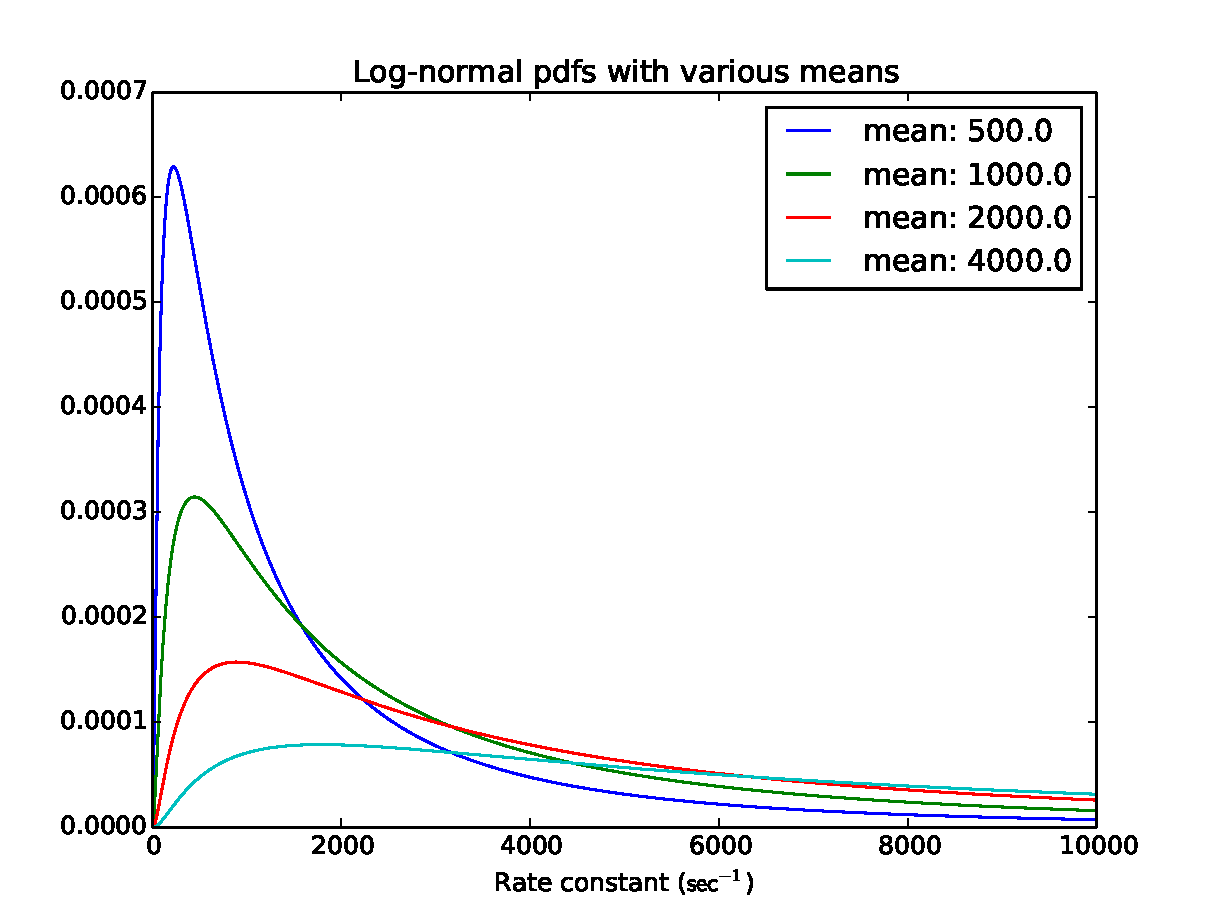
\includegraphics[width=\columnwidth]{lognorm_pdf_mean}
		\captionof{figure}{\label{fig:lognormalpdf-mean} The probability density functions of log-normal random variables with different coefficients of variation. Here, each log normal distribution has a fixed coefficient of variation of $2$.}
		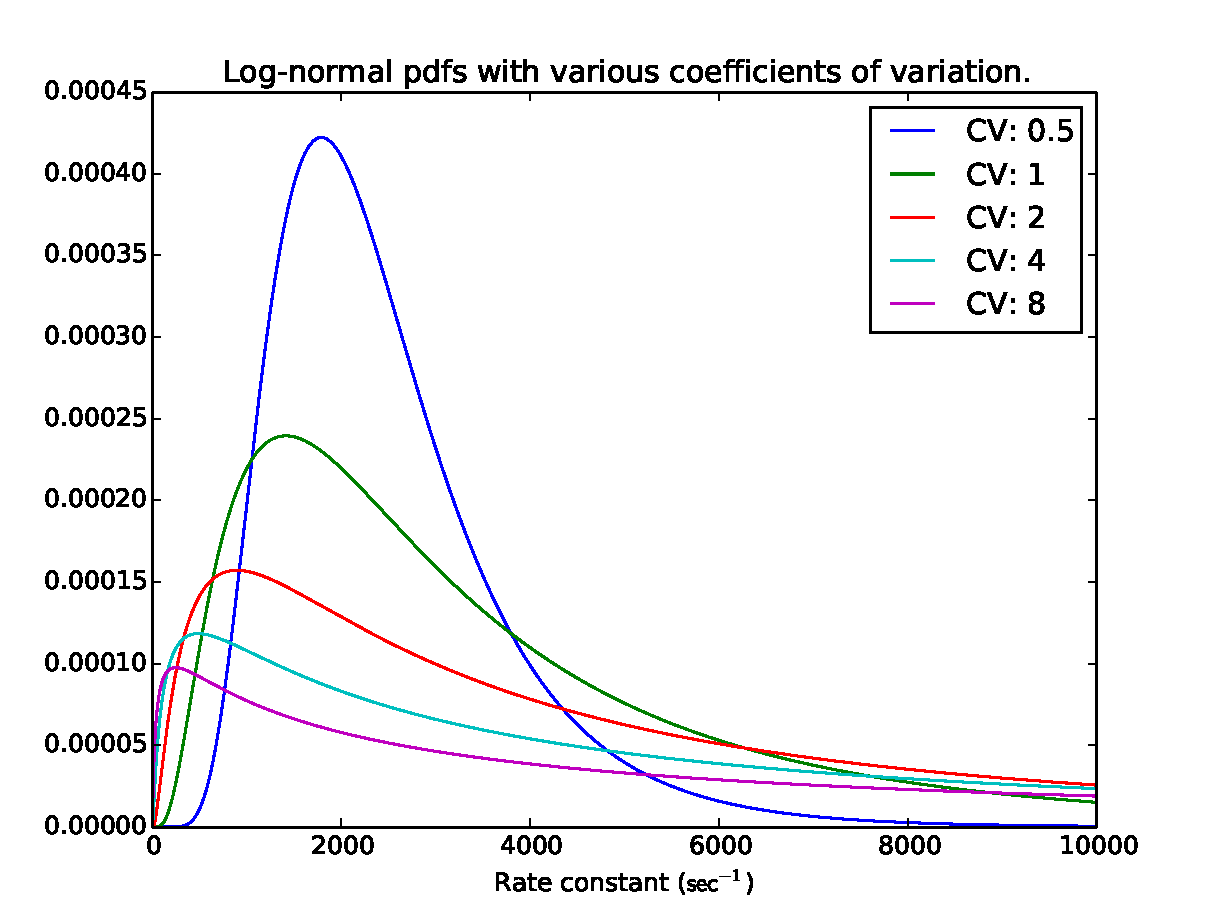
\includegraphics[width=\columnwidth]{lognorm_pdf_cvs}
		\captionof{figure}{\label{fig:lognormpdf-cvs}The probability density functions of log-normal random variables with different coefficients of variation. Here, each log normal distribution has a fixed mean of $2000\;\mathrm{sec}^{-1}$.}
	\end{infobox}
	\newpage
	
	For the purpose of simulation, in is convenient to approximate the integral \ref{eqn:total-current-disp} in terms of a weighted sum of $I_\mathrm{tot}(T, E_0, k_0)$ at particular quadrature points:
	\begin{equation}\label{eqn:disp-quadrature}
		I_{tot}(t) \approx \sum_{i=1}^N \sum_{j = 1}^M w_{i,j} I_{tot}(t, E_{0,i}, k_{0,j}).
	\end{equation}
	because $E_0$ and $\log k_0$ are normally distributed, it is computationally efficient to choose $E_{0,i}$, $k_{0,j}$, and $w_{i,j}$ in terms of the Gauss-Hermite quadrature points and weights.  In particular, the quadrature points are given by 
	\begin{equation}
		\begin{aligned}
			E_{0,i} &= \overline{E_0} + \sqrt{2} \sigma_{E_0} x_{i,N}\\
			k_{0,j} &= \overline{k_0} \exp(-\sigma_{\log k_0}^2 / 2) \exp\left(\sqrt{2} \sigma_{\log k_0} x_{j,M}\right)
		\end{aligned}
	\end{equation}
	and the weights by
	\begin{equation}
		w_{i,j} = \frac{w_{i,N}w_{j,M}}{\pi}
	\end{equation}
	where $x_{i,N}$ is the $i$th quadrature point of the $N$ point Guass-Hermite quadrature and $w_{i,N}$ is the associated quadrature weight.  The parameters $\overline{E_0}$ and $\overline{k_0}$ are the means of $E_0$ and $k_0$, respectively, and $\sigma_{E_0}$ and $\sigma_{\log k_0}$ denote the standard deviations of $E_0$ and $\log k_0$.  The value $\sigma_{\log k_0}$ is related to the coefficient of variation of $k_0$ by
	\begin{equation}
		%\begin{aligned}
		%	\CV[k_0] &= \sqrt{\exp(\sigma_{\log k_0}^2) - 1}\\
			\sigma_{\log k_0} = \sqrt{\log(1 + \CV[k_0] ^2)}
		%\end{aligned}
	\end{equation}
	
	\section{Number of points required to accurately simulate reactions with dispersion}
	
	To use \cref{eqn:disp-quadrature} to simulate a reaction with dispersion, it is necessary to choose the number of quadrature points $N$ and $M$ large enough to ensure a small error.  We conducted a numerical experiment to determine the number of points needed to achieve a relative error of at most $1\%$ in the time domain and the first $12$ harmonics.  In this experiment, we took a simulated current trace with $N = 85, M = 60$ points to represent the true current due to dispersion, and conducted a search over $N \le 85, M \le 60$ to find the least number of points needed to obtain the required tolerance.  The results are show in \cref{fig:thermo-disp,fig:kin-disp,fig:both-disp}.  
	
	From the figures, we see that it takes a greater number of points to resolve thermodynamic dispersion than it does to resolve kinetic dispersion.  \Cref{fig:both-disp} shows that $N$ depends only weakly on the level of kinetic dispersion and $M$ depends only weakly on he level of thermodynamic dispersion.
	
	\begin{figure}[h]
		\centering
		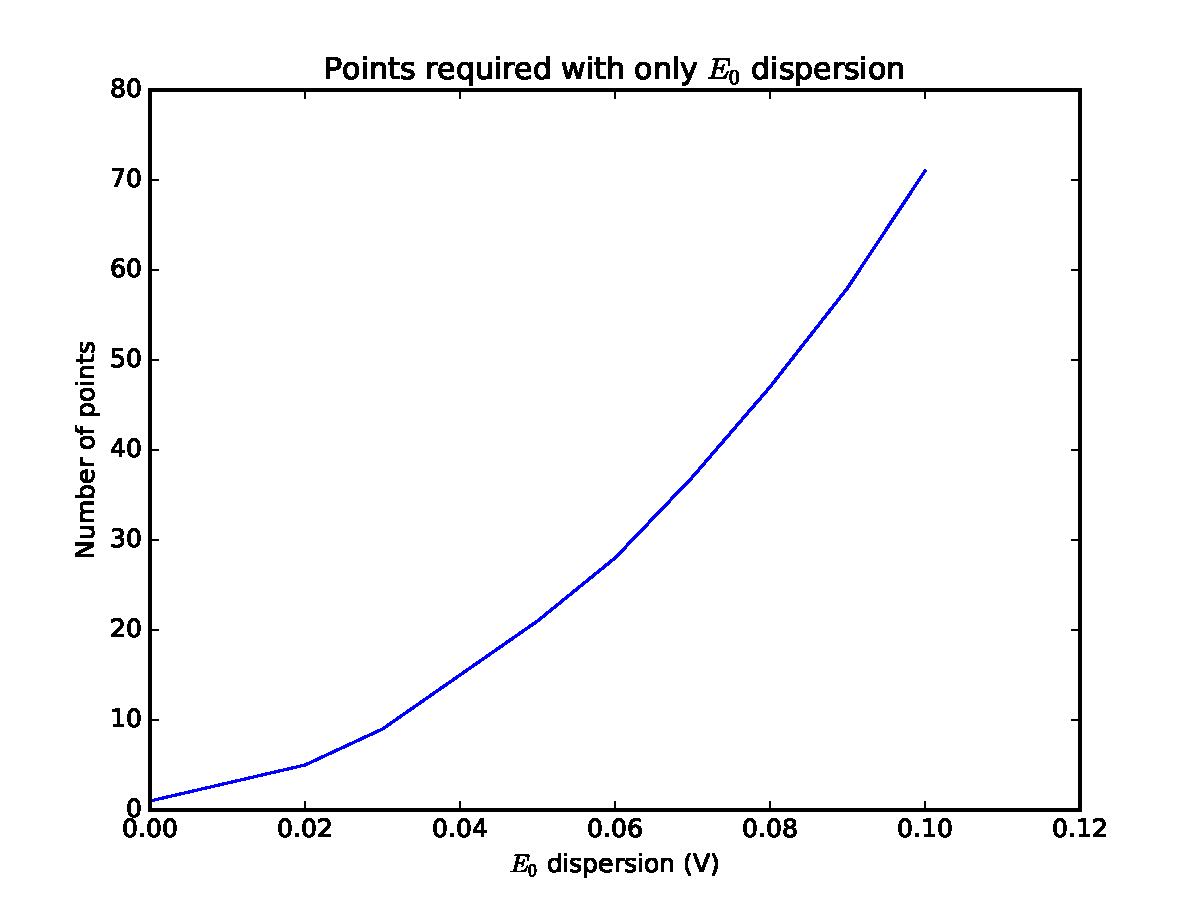
\includegraphics[height=6cm]{E0DispPts.pdf}
		\caption{\label{fig:thermo-disp} The number of points $N$ required to simulate a reaction with a given thermodynamic dispersion with an error of less than $1\%$. (given in terms of $\sigma_{E_0}$).  There is no kinetic dispersion, and the true current due to the reaction is taken to be the one produced using $N = 85$.}
	\end{figure}
		
	\begin{figure}[h]
		\centering
		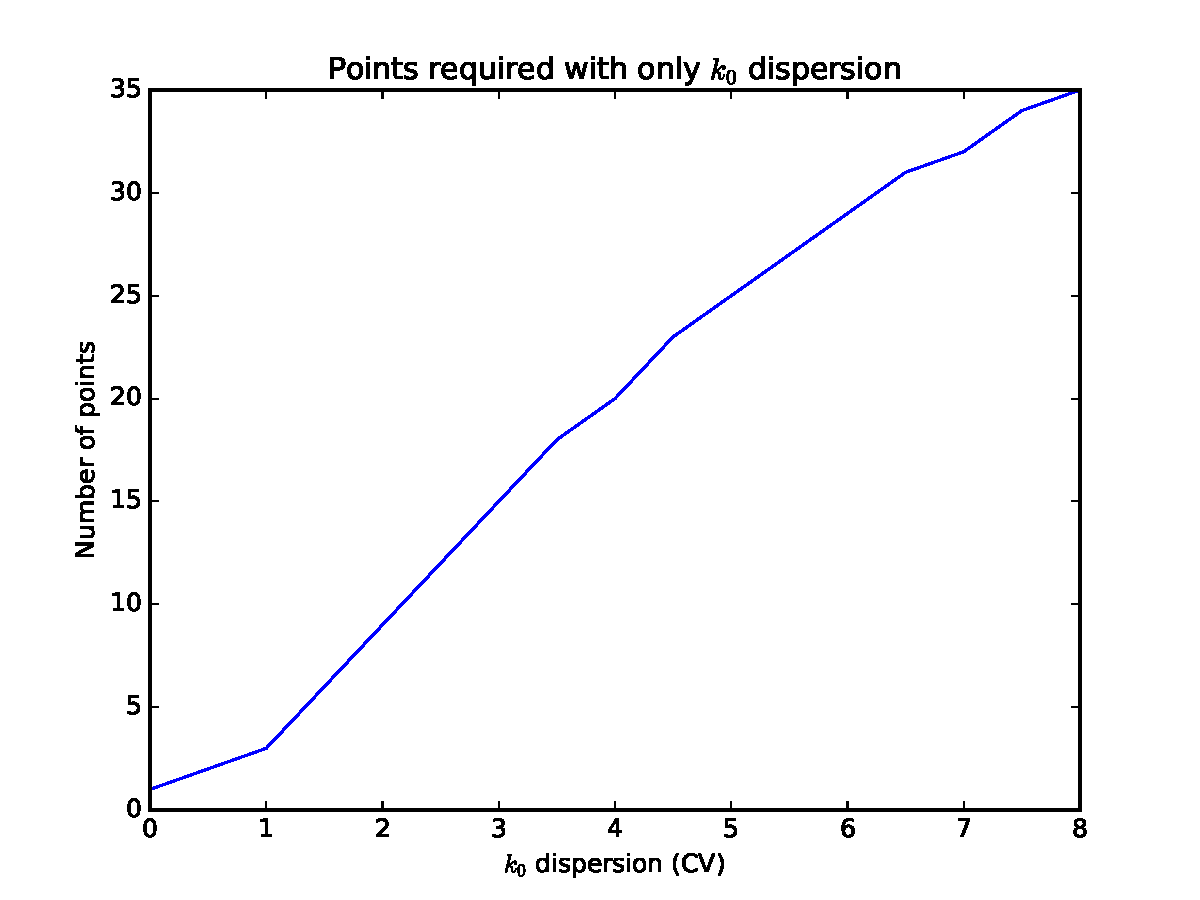
\includegraphics[height=6cm]{k0DispPts.pdf}
		\caption{\label{fig:kin-disp} The number of points $M$ required to simulate a reaction with a given kinetic dispersion with an error of less than $1\%$. (given in terms of $CV[k_0]$).  There is no thermodynamic dispersion, and the true current due to the reaction is taken to be the one produced using $M = 60$.}
	\end{figure}
		
	\begin{figure}[h]
		\centering
		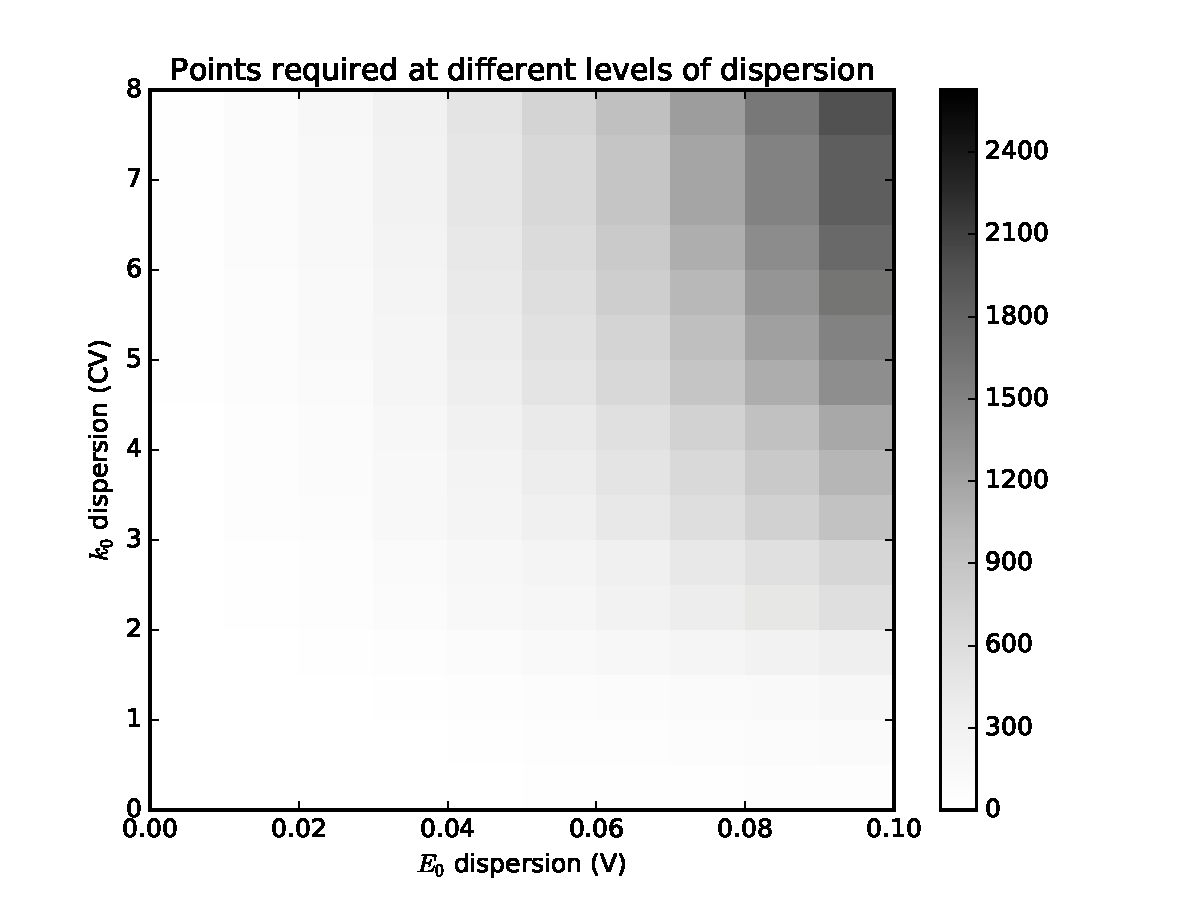
\includegraphics[height=6cm]{bothDispPts.pdf}
		\caption{\label{fig:both-disp} The number of points required to simulate, with an error of at most $1\%$, for varying levels of thermodynamic and kinetic dispersion.}
	\end{figure}
	
\end{document}